La organización por tareas del proyecto ha sido desglosada en una Estructura de Desglose de Trabajo o EDT que se muestra en la Figura \ref{fig:EDT}.

\begin{figure}[H]

    \makebox[\textwidth][c]{%
        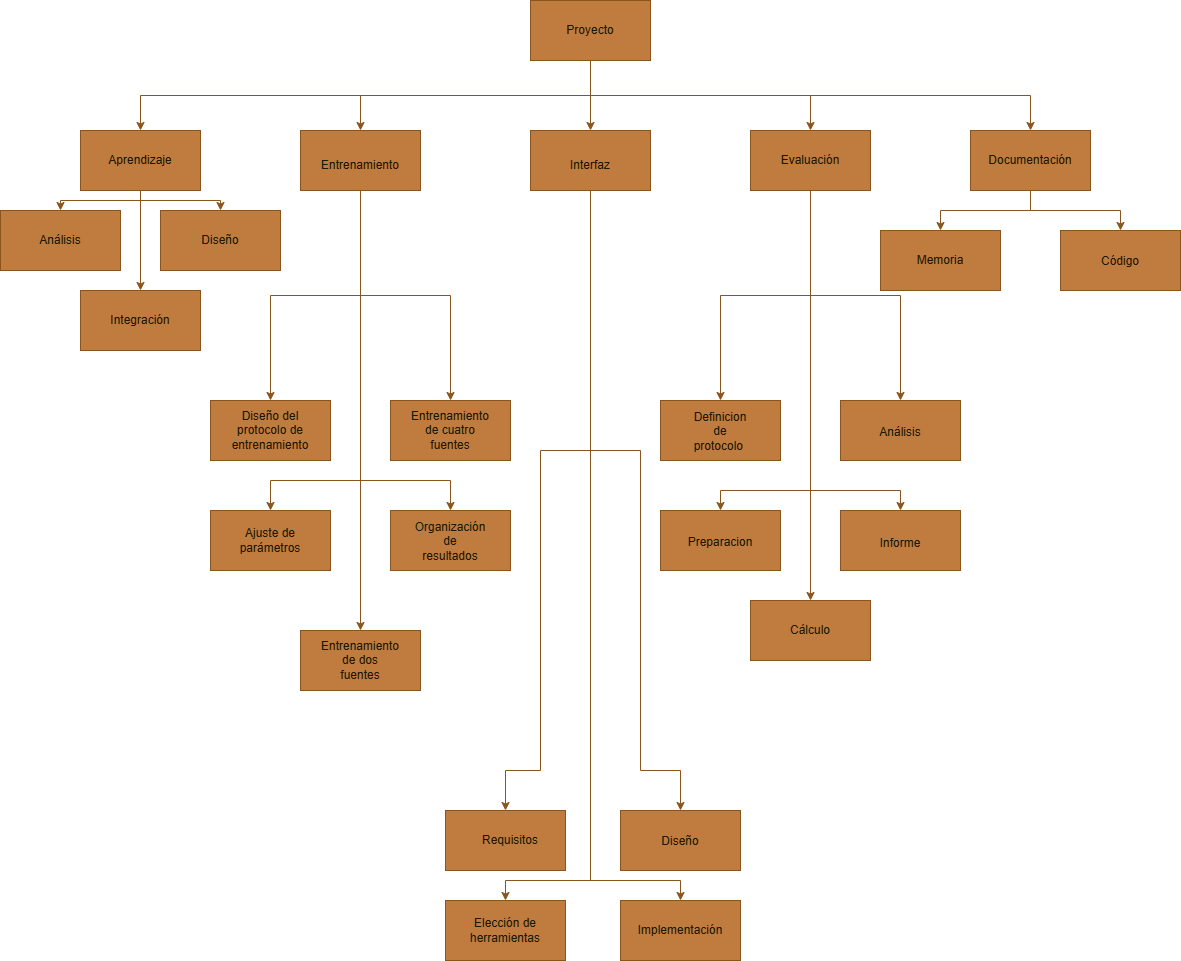
\includegraphics[
            width=1.50\textwidth,
            keepaspectratio
        ]{commons/EDT.png}%
    }

    \caption{Estructura de desglose de trabajo}
    \label{fig:EDT}
\end{figure}



Esta estructura está dividida en distintos paquetes de trabajo de la siguiente manera:

\begin{itemize}
    \item \textbf{PT 1.Aprendizaje y desarrollo inicial.}
    \begin{itemize}
        \item \textbf{T 1.1. Análisis del problema e investigación técnica.} 
        
        Estudio del problema de separación de fuentes, revisión de conceptos de audio digital y análisis de las herramientas necesarias para el desarrollo del sistema.
        \item \textbf{T 1.2. Implementación inicial en código de un modelo de separación de fuentes y de las funciones de pérdida.}
        
        Identificación de limitaciones y necesidades del proyecto, Implementación del modelo elegido de acuerdo a estas e incorporación de las funciones de pérdida propuestas.
        \item \textbf{T 1.3. Diseño del preprocesamiento.}
        
        Definición del proceso de preparación de los datos y transformación de señales.
    \end{itemize}
    \item \textbf{PT 2.Entrenamiento.}
    \begin{itemize}
        \item \textbf{T 2.1. Diseño del protocolo de entrenamiento.}
        
        Agrupación de muestras musicales elegidas en un conjunto de datos para entrenamiento y definición de estrategia para este , configuraciones evaluadas y criterios de comparación.
        \item \textbf{T 2.2. Ajuste de los parámetros de entrenamiento.}
        
        Estudio y elección de hiperparámetros. Integración de una configuración de estos para que se cumplan los requisitos de las dos variantes posibles del modelo planteadas a entrenar en las dos siguientes fases.
        \item \textbf{T 2.3. Entrenamiento de dos fuentes.}
        
        Entrenamiento de modelos orientados a separar una mezcla en voz y acompañamiento.
        \item \textbf{T 2.4. Entrenamiento de cuatro fuentes}
        
        Entrenamiento de modelos orientados a separar una mezcla en batería,voz,bajo y resto.
        \item \textbf{T 2.5. Organización de los resultados.}
        
        Recopilación, ordenación y preparación de los resultados generados durante los entrenamientos.
    \end{itemize}
    \item \textbf{PT 3.Implementación de la interfaz.}
    \begin{itemize}
        \item \textbf{T 3.1. Análisis de requisitos.}
        
        Definir funcionalidades que debe ofrecer la interfaz.
        \item \textbf{T 3.2. Elección de herramientas.}
        
        Seleccionar las tecnologías a utilizar en la implementación teniend en cuenta la facilidad de uso y la integración y compatibilidad con el sistema desarrollado.
        \item \textbf{T 3.3. Diseño del flujo.}
        
        Definir la secuencia de interacción del usuario con la aplicación.
        \item \textbf{T 3.4. Implementación.}
        
        Desarrollo de la interfaz, conexión con el modelo y validación de funcionalidades.
    \end{itemize}
    \item \textbf{PT 4.Evaluación.}
    \begin{itemize}
        \item \textbf{T 4.1. Definición de protocolo de evaluación.}
        
        Establecer cómo se van a evaluar los modelos, datos a utilizar y métricas a calcular.
        \item \textbf{T 4.2. Preparación de conjunto de evaluación }
        
        Seleccionar y organizar los audios a utilizar para medir el rendimiento final.
        \item \textbf{T 4.3. Cálculo de métricas.}
        
        Comprende el cálculo de métricas mediante scripts para cada modelo.
        \item \textbf{T 4.4. Análisis y representación de resultados.}
        
        Interpretación de resultados obtenidos, comparación entre modelos y elaboración de gráficas.
        \item \textbf{T 4.5. Elaboración de conclusiones y de trabajo futuro.}
        
        Recoger conclusión final en vista de los resultados y las limitaciones que estos presentan.
    \end{itemize}
    \item \textbf{PT 5. Documentación}
    \begin{itemize}
        \item \textbf{T 5.1. Redacción de la memoria.}
        
        Comprende escritura de la memoria y comunicación con los tutores para la corrección de esta. 
        \item \textbf{T 5.2. Documentación del código.}
        
        Revisión y limpieza del repositorio de código, organización de archivos y documentación básica.
    \end{itemize}
\end{itemize}